% -------------------------------------------------------------------------------
% Establish page structure & font.
\documentclass[12pt]{report}

\usepackage[total={6.5in, 9in},
	left=1in,
	right=1in,
	top=1in,
	bottom=1in,]{geometry} % Page structure

\usepackage{graphicx} % Required for inserting images
\graphicspath{{../.images/}} % Any additional images I use (BCU logo, etc) are from here.

\usepackage[utf8]{inputenc} % UTF-8 encoding
\usepackage[T1]{fontenc} % T1 font
\usepackage{float}  % Allows for floats to be positioned using [H], which correctly
                    % positions them relative to their location within my LaTeX code.
\usepackage{subcaption}
\usepackage{csquotes}

% -------------------------------------------------------------------------------
% Declare biblatex with custom Harvard BCU styling for referencing.
\usepackage[
    useprefix=true,
    maxcitenames=2,
    maxbibnames=99,
    style=authoryear,
    dashed=false, 
    natbib=true,
    url=false,
    backend=biber
]{biblatex}

\usepackage[british]{babel}

% Additional styling options to ensure Harvard referencing format.
\renewbibmacro*{volume+number+eid}{
    \printfield{volume}
    \setunit*{\addnbspace}
    \printfield{number}
    \setunit{\addcomma\space}
    \printfield{eid}}
\DeclareFieldFormat[article]{number}{\mkbibparens{#1}}

\addbibresource{Report.bib}

% -------------------------------------------------------------------------------
% To prevent "Chapter N" display for each chapter
\usepackage[compact]{titlesec}
\usepackage{wasysym}
\usepackage{import}

\titlespacing*{\chapter}{0pt}{-2cm}{0.5cm}
\titleformat{\chapter}[display]
{\normalfont\bfseries}{}{0pt}{\Huge}

% -------------------------------------------------------------------------------
% Custom macro to make an un-numbered footnote.

\newcommand\blfootnote[1]{
    \begingroup
    \renewcommand\thefootnote{}\footnote{#1}
    \addtocounter{footnote}{-1}
    \endgroup
}

% -------------------------------------------------------------------------------
% Fancy headers; used to show my name, BCU logo and current chapter for the page.
\usepackage{fancyhdr}
\usepackage{calc}
\pagestyle{fancy}

\setlength\headheight{37pt} % Set custom header height to fit the image.

\renewcommand{\chaptermark}[1]{%
    \markboth{#1}{}} % Include chapter name.


% Lewis Higgins - ID 22133848           [BCU LOGO]                [CHAPTER NAME]
\lhead{Lewis Higgins - ID 22133848~~~~~~~~~~~~~~~
\includegraphics[width=1.75cm]{BCU}}
\fancyhead[R]{\leftmark}

% ------------------------------------------------------------------------------
% Used to add PDF hyperlinks for figures and the contents page.

\usepackage{hyperref}

\hypersetup{
    colorlinks=true,
    linkcolor=black,
    filecolor=magenta,
    urlcolor=blue,
    citecolor=black,
}

% ------------------------------------------------------------------------------
\usepackage{xcolor} 
\usepackage{colortbl}
\usepackage{longtable}
\usepackage{amssymb}
% ------------------------------------------------------------------------------
\usepackage{tcolorbox}
\newcommand{\para}{\vspace{7pt}\noindent}
% -------------------------------------------------------------------------------

\title{IOThings Application Report}
\author{Lewis Higgins - Student ID 22133848}
\date{May 2025}

% -------------------------------------------------------------------------------

\begin{document}


\makeatletter
\begin{titlepage}
    \begin{center}
        
\includegraphics[width=0.7\linewidth]{BCU}\\[4ex]
        {\huge \bfseries CMP6207 - Assignment 1}\\[2ex]
        {\large \bfseries  \@title}\\[50ex]
        {\@author}\\[2ex]
        {CMP6207 - Modern Data Stores}\\[2ex]
        {Module Coordinator: Konstantinos Vlachos}\\[5ex]
    \end{center}
\end{titlepage}
\makeatother
\thispagestyle{empty}
\newpage


% Page counter trick so that the contents page doesn't increment it.
\setcounter{page}{0}

\tableofcontents
\thispagestyle{empty}

\chapter*{Introduction}
\addcontentsline{toc}{chapter}{Introduction}






% ? Chapter 1 - Types of NoSQL Databases.
\chapter{Types of NoSQL databases}
\noindent Structured Query Language, or SQL, was developed by IBM following \textcite{coddRelationalModelData1970}'s groundbreaking 
publication in the ACM journal, with the first commercial SQL implementation being published by Oracle in 1979 \autocite{oracleHistorySQL}.
SQL powers many relational database systems even today, though the problems associated with its age, most notably in 
the speed of its operations, are beginning to show in modern systems. Therefore, NoSQL ("Not Only SQL") was developed as 
an extension of SQL, allowing data to be stored in a non-tabular, non-relational format for efficient storage of
semi-structured and unstructured data in a flexible, functional and scalable model for faster operations than standard 
relational databases in most scenarios \autocite{googlecloudWhatNoSQLDatabases, awsWhatNoSQLDatabase}. There are a wide variety of NoSQL 
database types which vary in complexity, functionality and purpose, meaning that identification of the most suitable type is paramount 
for maximum efficiency. 

% TODO: Talk about ACID:
% ?     Atomicity - A statement is fully executed or not executed at all.
% ?     Consistency - Transactions only occur in predefined ways. (Helps prevent impacts of corruption)
% ?     Isolation - Concurrent transactions don't interfere with each other.
% ?     Durability - Changes are saved, even in the event of system failure. 
% *    https://www.databricks.com/glossary/acid-transactions
% ! Alternatively, talk about it in the comparison of relational & NoSQL.

\section{Document database}\label{sec:DocDBs}
% ? MongoDB is a document database.
% * General purpose databases.
Document databases are intuitive, flexible and horizontally scalable databases that work well in a wide variety of use cases
for both transactional and analytical purposes, including IoT data and real-time analytics \autocite{mongodbDocumentDatabaseNoSQL}.
They store records as "documents", which store an object's data and metadata, in a format such as JSON, BSON, or XML\footnote{JavaScript Object Notation, Binary JSON and Extensible Markup Language, respectively.}. Details and examples of these file types can be found in Appendix A.

% TODO: Finish Appendix A, where you talk about and give examples of each of these. See Lab 4 slides for modelling relationships with JSON.

\begin{figure}[H]
    \centering
    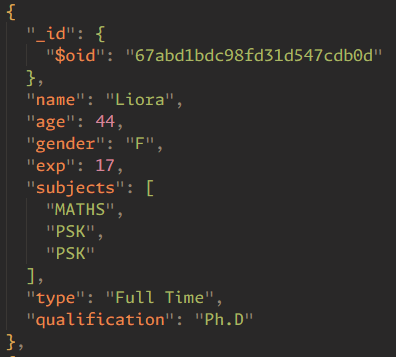
\includegraphics[width=0.7\textwidth]{NoSQL DBs/Doc/ExampleDoc}
    \caption{An example of a JSON Document.\label{fig:ExampleDoc}}
\end{figure}

\noindent Figure \ref{fig:ExampleDoc} depicts an example JSON document in MongoDB\footnote{MongoDB actually stores data as BSON, though it translates between the two when queried. See Appendix B for more information.}, a popular DBMS
for document databases. It contains the data of a singular example school teacher, storing details such as their name, age and subject expertise, as well as a unique internal object ID used by MongoDB to identify that document. The data itself is of varying types including 
strings, integers and arrays, which makes document databases easily integrable into a development workflow due to the direct 
storage of object types used in programming languages like Python and JavaScript.

% TODO: Has enough been written here?

\para Popular services for document databases include Databricks \autocite{databricksDataAICompany2023} Couchbase \autocite{couchbaseCouchbaseBestFree}, and the previously mentioned MongoDB \autocite{mongodbDocumentDatabaseNoSQL}.


\section{Key-value database}
% ? Redis is a key-value database.
% ! While that's true, it's also an in-memory database.
% * Very fast, very simple.
Key-value databases are primarily reputed for their speed and simplicity, functioning by storing each record as a key-value pair.
Rather than having to search through massive amounts of irrelevant data for a query, key-value databases can instead search 
through their stored keys to retrieve results within milliseconds or even microseconds if used in-memory \autocite{redisRedisFAQ}.
While this is excellent for simple queries to retrieve specific known records, this same property also causes major limitations in
that retrieving data based on values, such as finding all users over a given age, would require the entire database to be searched,
making key-value databases best suited for real-time data access and caching where simpler queries are used \autocite{mongodbWhatKeyValueDatabase}.

% TODO: You've spoke of key-value negatives here, so go back and do it for documents too.

\begin{figure}[H]
    \centering
    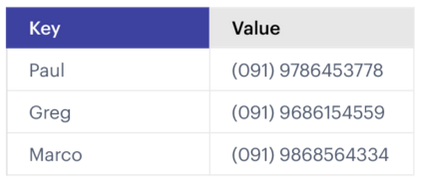
\includegraphics[width=0.5\textwidth]{NoSQL DBs/KeyValue/ExampleKeyVal}
    \caption{An example key-value pair \autocite{redisWhatKeyValueDatabase}.\label{fig:ExampleKeyVal}}
\end{figure}


\noindent Figure \ref{fig:ExampleKeyVal} depicts an example key-value pair, mapping names to phone numbers. If a query for "Greg" was given, 
the associated value would be returned. There is a significant similarity between key-value stores and document stores, though key-value stores
can only store simple key-value pairs, whereas document stores can have flexible schemas of complex, nested structures. Furthermore, as previously 
mentioned, querying key-value databases is very limited to only simple queries if speed is a decisive factor. 

\para Notable software options used across industry for key-value databases include Amazon's DynamoDB \autocite{awsFastNoSQLKeyValue}, Redis \autocite{redisWhatKeyValueDatabase}, and Memcached \autocite{memcachedMemcachedDistributedMemory}. MongoDB can also be used as a key-value store, though this is
not its primary intention.


\section{Column-oriented database}
% * Stores data in columns rather than rows.
% * Fast reading, slow writing. 
% * Better for OLAP than OLTP iirc.
% ! In the scenario, the slow writing means it's unwanted. Client wants IoT sensor data recorded, so it'll be lots of writing.
% ? Also known as wide-column stores, which may be the preferred term for the module spec.


\section{Graph database}
% ? Neo4J is a graph database.
% ! Target - Feb 23rd.


% ? Chapter 2 - Comparing NoSQL to Relational databases.
\chapter{Comparing NoSQL and Relational databases} 
% ! Chapter title doesn't fit the page.
\begin{itemize}
    \item This section "shouldn't be too long, but enough to convince them."
    \item \textbf{This is NOT comparing \textit{MongoDB} to relational databases.} The brief 
    mentions that it should be "generic just in case after seeing your MongoDB database they decide to go with another software provider."
\end{itemize}

% TODO: Talk about ACID:
% ?     Atomicity - A statement is fully executed or not executed at all.
% ?     Consistency - Transactions only occur in predefined ways. (Helps prevent impacts of corruption)
% ?     Isolation - Concurrent transactions don't interfere with each other.
% ?     Durability - Changes are saved, even in the event of system failure. 
% *    https://www.databricks.com/glossary/acid-transactions

% TODO: Talk about BASE:
% * A base is the opposite of an acid, hence the name.
% * Seems to be based on the *perception* of availability rather than the literal availability.
% ?     Basically Available - One transaction doesn't have to wait for another to complete first.
% ?     Soft State - The transitional state of records during concurrent updates. Finalised after all transactions complete.
% ?     Eventually Consistent - When all concurrent transactions are done, it will EVENTUALLY be consistent across all user perspectives.
% * https://aws.amazon.com/compare/the-difference-between-acid-and-base-database/

% TODO: Talk about the CAP theorem:
% ?     Consistency: Once data is written, it is available to all users of the system immediately.
% ?     Availability: The service is uninterrupted and without degradation for the majority of the time.
% ?     Partition Tolerance: Operations can be completed even if part of the network fails.

% TODO: Talk about horizontal scalability.
% ?     Why is vertical bad?
% ?     Nodes and sharding


% ! Target - Feb 25th/27th.


% ! If possible, keep work up to this point under ~2500 words perhaps. Remember the limit is 4,400 rather than 4,000 flat.
% TODO: Perhaps it won't be necessary yet, but you will have to account for the fact you've blown over this expectation already.

% ! Remember that TeXcount is currently counting your appendices. Comment them out for true count.


% ? Chapter 3 - Database Design and Implementation.
\chapter{Database design and implementation}

% MongoDB, an acronym from "hu\textbf{mongo}us \textbf{DB}", aims to address some of SQL's antiquation issues\dots

\section{Target problem}
\subsection{Clientele}
IoThings are a UK-based small-to-medium sized enterprise specialising in Internet of Things home automation systems.
Specifically, they install sensors and use MQ Telemetry Transport (MQTT) to collect their activation data and store it in 
a MongoDB database for analytical purposes. These sensors can be used for a variety of reasons, such as:

\begin{itemize}
    \item Temperature control
    \item Lighting control 
    \item Entertainment management 
    \item Home security
\end{itemize}

\subsection{Existing systems}
IoThings already have an extensive data storage solution for their Enterprise Resource Planning (ERP), Customer Relationship 
Management (CRM), finances, order processing / sales, and logistics. However, they do not presently have an optimal solution for 
their MQTT sensor activation data.  


\subsection{Requested solution}
Therefore, IoThings wish to extend their current data storage implementation with an additional NoSQL database to contain their 
sensor activation data for the eventual purpose of giving feedback to their users about device usage. In addition to the 
creation of this database, the client also requests the development of an API and frontend for accessing and processing the 
stored data.

\para Due to data security and privacy concerns, it is not possible for IoThings to provide data of their own. Therefore, 
the solution developed in this report will use synthetic data which aims to replicate the data which would theoretically 
be stored.


% ? Chapter 4 - API Implementation and Documentation.
\chapter{API Implementation and Documentation}


\chapter*{Conclusion}
\addcontentsline{toc}{chapter}{Conclusion}
% ! I want to be done with this report by April 14th, with the 
% ! April 29 - May 4 window being for final improvements, presentation prep, and other assignments.

Overall, something was done\dots

% ! FINAL TODOS BEFORE COMPLETION:
% ?     1.1 - Document databases: Footnote refers to "Appendix B". Is it still Appendix B by this point?
% ?     1.3 - Wide-column databases: Have you spoke about sharding before that section?
% ?     1.3 - Wide-column databases: You haven't spoke about normal column stores yet.
% ?     CAP Theorem - Where should it be mentioned? Chapter 1 or Chapter 2?
% !     Chapter 2 is woefully long. No chance that can escape a word count reduction.


% ?     Standard cleanup. Fit images and tables to pages, try not to break text over multiple in an ugly way.

% ! Additional notes (previously in introduction):
    % ? He wants you to make an Atlas account even if you do it locally?
    % ? You are creating the dataset for this assignment. You will describe it in an appendix rather than the report's main body.
        % ! The 4,400 word limit may therefore be deceptive, and you should not underestimate the workload of this report.
        
    % ? This is a "professional report", and as such the title page with the BCU logo and your info should probably change.
    % ? It needs to also show the date.

% ? Prevents bibliography overflowing hbox at the expense of it taking up more lines on the page.
\emergencystretch=1em

\printbibliography
\addcontentsline{toc}{chapter}{Bibliography}


% \begingroup
\renewcommand\thechapter{A}
\titleformat{\chapter}[display]
{\normalfont\huge\bfseries}{}{20pt}{\Huge}
\setcounter{section}{0}
\setcounter{figure}{0} 

\chapter*{Appendix A - Data types}
\addcontentsline{toc}{chapter}{Appendix A - Data types}

The types of data stored in databases vary dependent on their file format. Section \ref{sec:DocDBs} referred to three 
major file formats used in document databases - JavaScript Object Notation (JSON), Binary JSON (BSON), and Extensible Markup Language (XML).
Each of these have their own distinct attributes, which will be thoroughly described in this appendix.

\section{JavaScript Object Notation (JSON)}
JSON files are\dots

\section{Binary JSON (BSON)}
BSON files are\dots

\section{Extensible Markup Language (XML)}
XML files are\dots

\endgroup
% \begingroup
\renewcommand\thechapter{B}
\titleformat{\chapter}[display]
{\normalfont\huge\bfseries}{}{20pt}{\Huge}
\setcounter{section}{0}
\setcounter{figure}{0} 

\chapter*{Appendix B - MongoDB and VS Code}
\addcontentsline{toc}{chapter}{Appendix B - MongoDB and Visual Studio Code}

Throughout the course of this project's development, Visual Studio Code ("VSCode") was used as the IDE.
VSCode allows its features to be expanded through extensions on its community marketplace. To assist greatly with 
this project's development, the MongoDB VSCode extension was installed, which provides the interface shown in 
Figure \ref{fig:VSCodeMongoUI}

\begin{figure}[H]
    \centering
    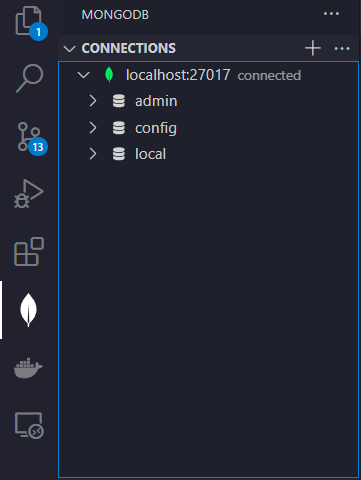
\includegraphics[width=0.5\textwidth]{VSCode/MongoExtensionUI}
    \caption{The MongoDB extension interface within VSCode.\label{fig:VSCodeMongoUI}}
\end{figure}


% This maybe doesn't actually have to be an appendix, though I wasn't sure where would be best to address this topic.
% Consider that it also doesn't really need addressing at all unless you use a hyper-specific feature.

\endgroup



\end{document}